\documentclass{beamer}
\usetheme{Hannover}

\usepackage{tikz}
\usetikzlibrary{positioning}
\usetikzlibrary{shapes}


\usepackage{algorithm}
\usepackage{algorithmic}
\usepackage{amsmath}
\usepackage{amssymb}
\usepackage{amsthm}
\usepackage[ngerman,english]{babel}
\usepackage{centernot} 
\usepackage{color}
\usepackage{dsfont}
\usepackage{graphicx}
\usepackage[utf8]{inputenc}
\usepackage{import}
\usepackage{standalone}
\usepackage{qtree}

\usepackage{hyperref}

\title{SOP Challenge - Presentation}
\author{TBD}

\newcommand{\N}{\ensuremath{\mathds{N}}}
\newcommand{\R}{\ensuremath{\mathds{R}}}
\newcommand{\red}[1]{\textcolor{red}{#1}}

\setlength{\itemsep}{-2pt}


\begin{document}
	 % --- frame 1 ---
	\begin{frame}{\textbf{P}article \textbf{S}warm \textbf{O}ptimization}
		\begin{columns}
			\column{0.5\textwidth}
				\begin{itemize}
					\item Used for multimodal functions
					\item Population based
					\item Iterative algorithm	
				\end{itemize}
			\column{0.5\textwidth}
				\begin{figure}[htp]
					\centering
					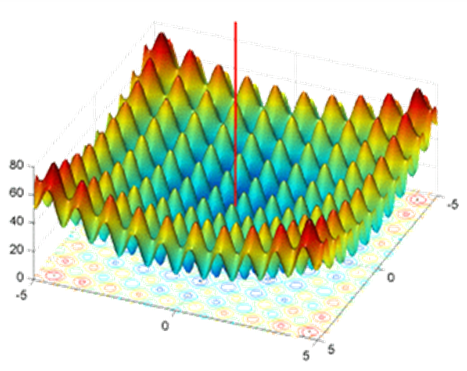
\includegraphics[width=5cm,height=5cm]{images/dpso_rastrigin.png}
					\caption{Example of multimodal function - Rastrigin}
				\end{figure}
		\end{columns}
	\end{frame}
	
	 % --- frame 2 ---
	\begin{frame}{\textbf{P}article \textbf{S}warm \textbf{O}ptimization}
		\begin{figure}[htp]
			\centering
			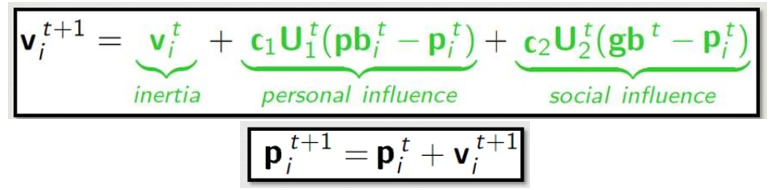
\includegraphics[width=\textwidth]{images/dpso_formula_vertical.png}
			\caption{PSO update formula}
		\end{figure}
	
		\begin{columns}
			\column{0.5\textwidth}
				\begin{itemize}
					\item Particles are vectors of coordinates
					\item Velocities are coordinate-wise
					\item Feasibility of particles is guaranteed
				\end{itemize}
			\column{0.5\textwidth}
				\begin{figure}[htp]
					\centering
					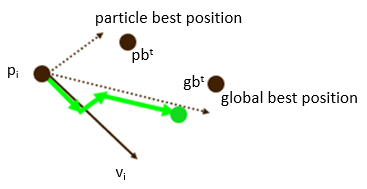
\includegraphics[width=\textwidth]{images/dpso_update.png}
					\caption{PSO update}
				\end{figure}
		\end{columns}
	\end{frame}

	% --- frame 3 ---
	\begin{frame}{\textbf{D}iscrete \textbf{P}article \textbf{S}warm \textbf{O}ptimization}
	
		\begin{itemize}
			\item Particles are permutations
			\item Velocities are pairs $ (n, d) $:
				\begin{itemize}
					\item $ n $ = node
					\item $ d $ = left/right displacement
				\end{itemize}
		\end{itemize}
	
		\begin{figure}[H]
			\centering
			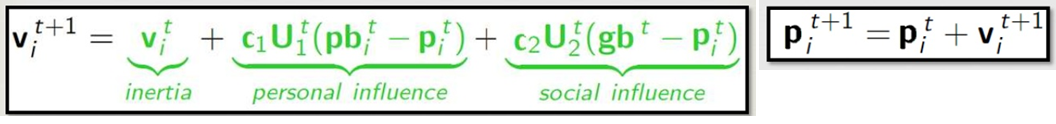
\includegraphics[width=\textwidth]{images/dpso_formula_horizontal.png}
		\end{figure}
		
		\begin{itemize}
			\item $ pA - pB $: velocities to $ pB $ to obtain $ pA $
			\item $ const * velocity $: delete or modify elements in $ velocity $
			\item $ perm + velocity $: modify $ perm $ with moves in $ velocity $
		\end{itemize}
		
		\medskip
			
		\begin{columns}
			\column{0.40\textwidth}
				%\centering Particles may NOT be feasible
				\centering Feasibility of particles is \textcolor{red}{NOT} guaranteed
			\column{0.02\textwidth}
				$ \Rightarrow $
			\column{0.58\textwidth}
				\centering modify permutation to respect precedence constraints \\ (\textcolor{red}{very slow})
		\end{columns}
		
	
	\end{frame}

\end{document}